\chapter{圧縮ベースパターン認識}
% 本章では,既存の圧縮ベースパターン認識手法を紹介する.

本章では,はじめに圧縮ベースパターン認識で利用される圧縮アルゴリズムである,LZWについて説明し,
その後,圧縮後のファイルサイズを利用する手法と圧縮辞書から特徴抽出する手法それぞれについて述べる.
圧縮ベースパターン認識は,ツイッターデータ~\cite{Nishida:2011:TCD:2064448.2064473},音楽~\cite{Wolf04algorithmicclustering},画像解析~\cite{Li2006}~\cite{e15010407},バイオインフォマティクス~\cite{li2001information}~\cite{1405274}など,1次元に表現されたデータであれば何でも解析可能という利点がある.

\section{LZW圧縮アルゴリズム}
この章では,本研究でオブジェクトの符号化と辞書の作成に用いる,LZW圧縮アルゴリズム~\cite{Welch:1984:THD:1319729.1320134}について詳しく述べる.
LZWでは,高速かつ高い圧縮効率を追求しており,現在もGIF画像やTIFF画像などの圧縮に用いられている圧縮アルゴリズムである.

LZW符号化の手順について説明する.
符号化では,圧縮されたテキストと復号に用いられる辞書が得られるが,
本研究ではこの辞書を利用している.なお,ここでは
圧縮元のテキストは8bitの記号を前提として説明する.

\begin{table*}[tb]% Table 1
\caption{初期状態のLZW辞書.}
%\ecaption{Comparison of correlation coefficient between baseline(upper right) and proposed(lower left) method(bold letter indicate  that absolute value of  correlation coefficient is less than 0.4 in the cell).}
\label{lz}
\begin{center}
\scalebox{1}{
\begin{tabular}{r|r  }
\hline
単語 & 符号 \\
\hline
(0) & 0 \\
(1) & 1 \\
\vdots & \vdots \\
(255) & 255 \\
\hline
\end{tabular}%
}
\end{center}
\end{table*}

\begin{description}
	\item [Step1] 8bitの256種類の全記号を登録した辞書を用意する.ここで,記号を8bitの整数として扱った場合の整数値をその単語の符号とする(表\ref{lz}).
	さらに,最長一致文字列とその符号を記憶する領域(バッファ)を確保する.

	\textgt{
	バッファの状態:最長一致文字列 = (空),符号 = (空)
	}
	\item [Step2] テキストの最初の記号を読み込んで最長一致文字列とし,
	それを整数として扱った値を符号として記憶する.
	例えば最初の記号が'a'で,その整数値が97とするとバッファの内容はつぎのようになる.

	\textgt{
	バッファの状態:最長一致文字列 = a,符号 = 97
	}
	\item [Step3] 次の記号を読み込み,その記号を最長一致文字列に
	追加した「現在の最長一致文字列+読み込んだ記号」という単語を
	辞書から探して,以下のいずれかの処理をおこなう.
	\begin{description}
		\item [(a)単語が辞書にある]
		その単語を最長一致文字列にして,その符号を記憶する.
		この操作を,「現在の最長一致文字列+読み込んだ記号」が辞書にない記号列になるまで繰り返す.
		\item [(b)単語が辞書にない]現在の最長一致文字列の符号を出力し,記号列を新しい単語として辞書に登録する.Step4へ.
	\end{description}
	例えばバッファの状態がつぎのようになっているとする.

	\textgt{
	バッファの状態:最長一致文字列 = c$\cdots$b,符号 = 312
	}

	このとき,次に読み込んだ記号を'c'として「c$\cdots$bc」が辞書にない場合,
	現在の最長一致文字列c$\cdots$bの符号を出力する($312_{(10)}$ = $100111000_{(2)}$).そして,記号列c$\cdots$bcを新しい単語として辞書に登録
	する.仮に,記号列c$\cdots$bcの符号を410とすると,登録後の辞書は
	表\ref{lz2}のようになる.

	\item [Step4] 今読み込んだ記号をあらためて最長一致文字列として,その整数値の符号を記憶する.前のステップの例をそのまま用いると,バッファの状態はつぎのようになる.

	\textgt{
	バッファの状態:最長一致文字列 = c,符号 = 99
	}

	\item [Step5] オブジェクト列が終了するまで,Step3$\sim$Step4を繰り返す.

\end{description}

\begin{table*}[tb]% Table 1
\caption{単語を登録した後のLZW辞書.}
%\ecaption{Comparison of correlation coefficient between baseline(upper right) and proposed(lower left) method(bold letter indicate  that absolute value of  correlation coefficient is less than 0.4 in the cell).}
\label{lz2}
\begin{center}
\scalebox{1}{
\begin{tabular}{r|r  }
\hline
単語 & 符号 \\
\hline
(0) & 0 \\
(1) & 1 \\
\vdots & \vdots \\
(255) & 255 \\
\vdots & \vdots \\
c$\cdots$b & 312 \\
\vdots & \vdots \\
c$\cdots$bc & 410 \\
\hline
\end{tabular}%
}
\end{center}
\end{table*}



\section{圧縮後のファイルサイズを利用する手法}
\subsection{基本的な考え}
%中島先輩の論文から引用
現在用いられている,圧縮後のファイルサイズ(圧縮率)を用いた手法の基本となる
概念はコルモゴロフ複雑性(Kolmogorov Complexity)\cite{osamu2006}が基となっている.
コルモゴロフ複雑性は,有限長のオブジェクト列の複雑度を表す指標であり,
与えられた文字列$x$に対してのコルモゴロフ複雑性$K(x)$はつぎのように定義される.
\begin{equation}
K(x) = \min_{q \in Q_x} |q| \label{kol}
\end{equation}
これは文字列$x$を出力可能なプログラム集合$Q_x$において,
この中で最小の文章量をもつプログラム$q$の長さが$K(x)$となる.
この値が大きいほど,その文字列は複雑と解釈される.

例として,つぎの2つの入力文字列を考える.
\begin{verbatim}
文字列1:xwxwxwxwxwxwxwxwxwxw
文字列2:3s2sm6br4z2f9cfd8jza
\end{verbatim}
これらの文字列を出力するプログラムを考えた時,
前者は「xwを10回出力」に対し,後者は
特に規則性をもたないので「3s2sm6br4z2f9cfd8jzaを出力」
と書く他はないように思える.
この場合,文字列を出力するプログラムの長さは後者のほうが長いので,
文字列2は文字列1より複雑であると考えられる.このようにコルモゴロフ複雑性では,
文字列を説明するプログラムの長さは,文字列そのものの複雑さと関係していることを
示している.

以上で説明した式(\ref{kol})は,プログラムが単独で$x$を生成する場合の定義である.
さらに,$y$に対する$x$の相対的コルモゴロフ複雑性を$K(x|y)$をつぎのように定義する.
\begin{equation}
K(x|y) = \min_{q(y) \in Q_x} |q(y)| \label{kol2}
\end{equation}
これは,$y$という補助オブジェクトを入力として,$x$を生成する
プログラムの最小長である.
一般的に,$y$に含まれる情報を用いる場合はより短いプログラムで$x$
が生成できる.したがって,$K(x|y)$は$K(x)$よりも小さくなる可能性がある.
この時に$K(x)$,$K(x|y)$の差$K(x)-K(x|y)$は,
$x$を予備知識なしに圧縮する場合に対し,$y$を仮定して
圧縮する場合の「改善度」を表す.すなわち,$K(x)-K(x|y)$は
$x,y$両者の類似部分の量と解釈することができる.

以上に説明したコルモゴロフ複雑性は計算不能として知られており,実際に
は用いることはできない.
そこで実用的には,データ圧縮技術を用いてオブジェクトの情報量や
オブジェクト間の類似性を評価している.

オブジェクト自身の複雑度を評価する場合は,そのオブジェクトを圧縮した時の
圧縮率で判断する.ただし,圧縮率はつぎのように定義される.
\begin{equation}
圧縮率 = \frac{圧縮後のファイルのサイズ}{圧縮前のファイルのサイズ}
\end{equation}
以上の定義から,圧縮率が大きい場合はそのオブジェクトの圧縮効率が悪いことが分かる.
つまり,圧縮率が大きい場合はオブジェクトは複雑であり,小さい場合はオブジェクトは単純
であると解釈できる.

例として,先ほど挙げた2つの文字列をUNIX標準のcompressコマンド
によって圧縮した結果を示す.

\begin{verbatim}
文字列1:xwxwxwxwxwxwxwxwxwxw を圧縮した場合
~$compress -f -v string1.txt
string1.txt:  -- replaced with string1.txt.Z Compression: 33.33%
文字列2:3s2sm6br4z2f9cfd8jza を圧縮した場合
~$compress -f -v string2.txt
string2.txt:  -- replaced with string2.txt.Z Compression: -28.57
\end{verbatim}
なお,出力におけるCompressionは圧縮効率(何\%削減できたか)を表す.
結果を見ると,文字列1は規則的なパターンをもつ単純な文字列なので,
圧縮ができていることがわかる.対して,文字列2は不規則なパターンをもつ
文字列であり,圧縮が上手くできておらず圧縮前よりもサイズが上回っていることがわかる.
このように,コルモゴロフ複雑性と同様に,テキストの複雑さとその圧縮率には関係性があり,
データ圧縮によって評価できることが分かる.

つぎにデータ圧縮技術によってオブジェクト間の類似度を評価する考え方について説明する.
オブジェクト$x,y$が似ているかどうか調べる場合,まずオブジェクト$y$の情報を用いて
,もう一方のオブジェクト$x$の圧縮をおこなう.

この処理を具体的に説明する.
はじめに,$y$を圧縮することで得られる辞書を作成する(図\ref{dic}).
\begin{figure}[tb]
\begin{center}
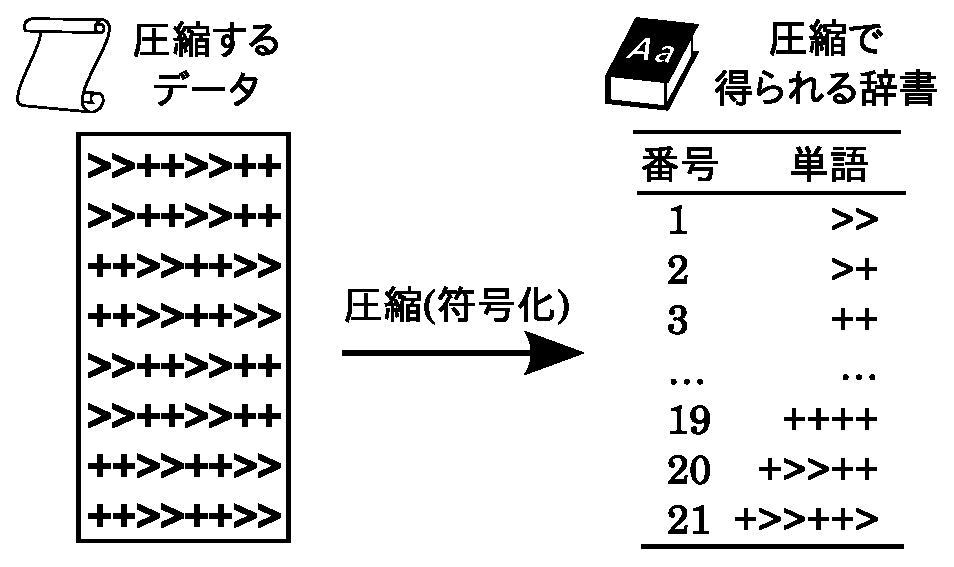
\includegraphics[width=10.5cm]{image/dic.eps}
\end{center}
\caption{データ圧縮によって得られる辞書.}
\label{dic}
\end{figure}
この辞書は圧縮対象のオブジェクトに頻出するパターンを保持していることがわかる.
そしてこの$y$の辞書を用いて,$x$を圧縮することで圧縮率を求める.
この圧縮率が
大きい場合には,$y$は$x$と類似するパターンを持っていないので,似ていないと解釈できる.
逆に圧縮率が小さい場合には,$y$は$x$と類似するパターンを多く持っているため,
似ていると解釈できる.

まとめると,オブジェクトに対する圧縮率の大小はつぎのように定義できる.
\begin{description}
	\item [圧縮率が大きい] オブジェクトのランダム性が高い $\Rightarrow$ 複雑なオブジェクト
	\item [圧縮率が小さい] オブジェクトのランダム性が低い $\Rightarrow$ 単純なオブジェクト
\end{description}
以上がデータ圧縮技術を用いた,オブジェクトの解析方法である.


\subsection{Normalized Compression Distance(NCD)}
\label{subsec:NCD}

NCD \cite{NCD} は2つのオブジェクト$x,y$間の距離を圧縮後のファイルサイズから算出する手法である.
$x,y$間の距離 NCD($x,y$)は式\ref{eq:NCD}のように定義される.
\begin{eqnarray}
\mathrm{NCD}(x,y) = \frac{C(xy) - \min\{C(x),C(y)\}}{\max\{C(x),C(y)\}} \label{eq:NCD}
\end{eqnarray}
ここで$C(x)$はオブジェクト$x$を圧縮したときのファイルサイズ,また$C(xy)$はオブジェクト$x,y$を連結した
$xy$を圧縮したときのファイルサイズを表す.$x,y$が類似しているほど$xy$がよりコンパクトに圧縮できるので,
$\mbox{NCD}(x,y)$は小さくなる.

NCDでは,図\ref{ncd}のようにオブジェクト$x$と$y$で共通するパターンが
多い場合に$C(xy)$は小さくなる.対して,$x$と$y$で共通するパターンが
少ない場合には$C(xy)$は大きくなる.このような性質を持っている.

\begin{figure}[tb]
\begin{center}
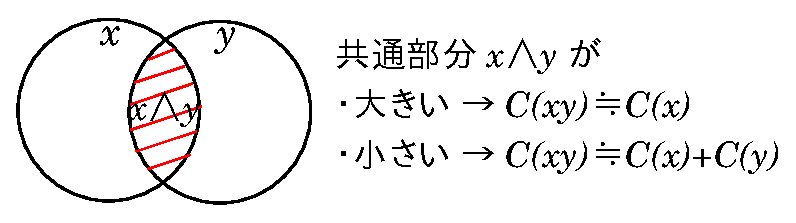
\includegraphics[width=13.5cm]{image/ncd.eps}
\end{center}
\caption{NCDの性質.}
\label{ncd}
\end{figure}

式(\ref{eq:NCD})から分かるように,NCDは計算において,パラメータを必要としない
パラメータフリーな手法といった利点がある.
しかし,NCDでは類似度の計算の度に$xy$の圧縮計算が必要である.
仮に文字列$x$,文字列$y$の文字数をそれぞれ$n_x, n_y$とし,
$x$から抽出される辞書の単語数を$m_x$,$y$から抽出される辞書の単語数を$m_y$として,$C(xy)$の計算量を考える.
なお,辞書の単語は辞書式順にソートされているとする.
このとき,オブジェクト$xy$の圧縮を考えると,最大でサイズが$m_x + m_y$の辞書に対して二分探索を
して単語を探す操作を,$n_x + n_y$回おこなう必要がある.
したがって,$C(xy)$の計算量は$(n_x + n_y)\log(m_x + m_y)$と表せる.

NCDをデータ集合の分類に適用した場合,データペア間の距離行列の計算が必要である.
この距離行列の計算量はデータベースに登録されているデータ数の2乗オーダとなる.
この為NCDでは,データの数が100個を超えるようなデータセットへの適用が難しい
という問題がある.




\subsection{PRDC}
PRDC \cite{PRDC} では,圧縮率ベクトルと呼ばれる特徴量によりオブジェクトを表現して,分類や類似検索を実現する.
PRDCはオブジェクトを特徴ベクトルとして扱うので,NCD等の距離尺度と比べると,$k$-means法や
SVM(Support Vector Machine)などベクトルベースのパターン認識手法の利用に適する.

PRDCでは,$N$個の基底辞書集合$B=\{D_1,D_2,\dots,D_N\}$を最初に定める.そして,オブジェクト$x$を
それぞれの辞書で圧縮した$N$次元の圧縮率ベクトルとして$x$を表現する.(図\ref{fig:PRDC.eps})
\begin{figure}[tb]
\centering
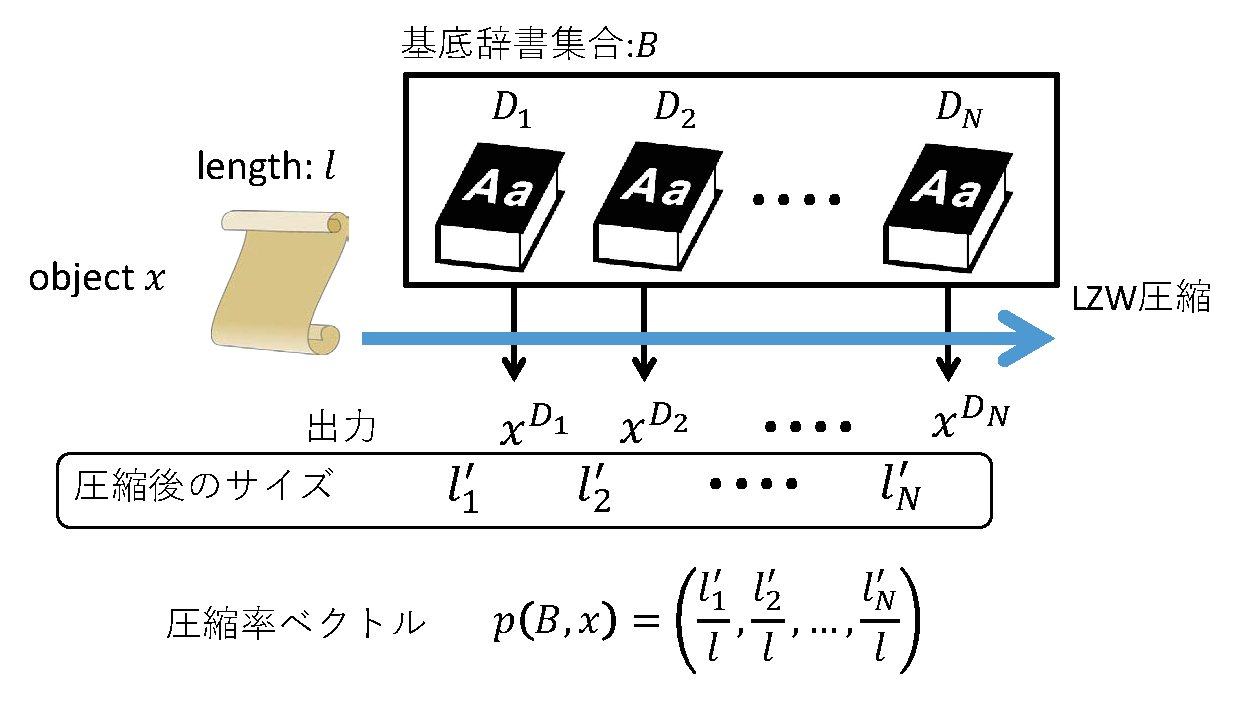
\includegraphics[clip, width=\columnwidth]{image/PRDC.eps}
\caption{圧縮率ベクトルの作成}
\label{fig:PRDC.eps}
\end{figure}

圧縮率ベクトル$\boldsymbol{p}(B,x)$はつぎのように定義される.

\begin{equation}
\boldsymbol{p}(B,x) = \biggl(\frac{l'_1}{l}, \frac{l'_2}{l},\dots,\frac{l'_N}{l} \biggr).
\label{eq:PRDC}
\end{equation}
長さ$l$の入力オブジェクト$x$が与えられた時,$x$をそれぞれの基底辞書により圧縮すると,
出力長$l'_1,l'_2,\dots,l'_N$が得られる.それぞれの出力長を元のオブジェクト長$l$で割った圧縮率を
並べたのが圧縮率ベクトルとなる.ここで出力長とは圧縮後のファイルサイズに他ならず,
PRDCも圧縮後のファイルサイズを利用する手法と位置づけられる.

\begin{figure}[tb]
\begin{center}
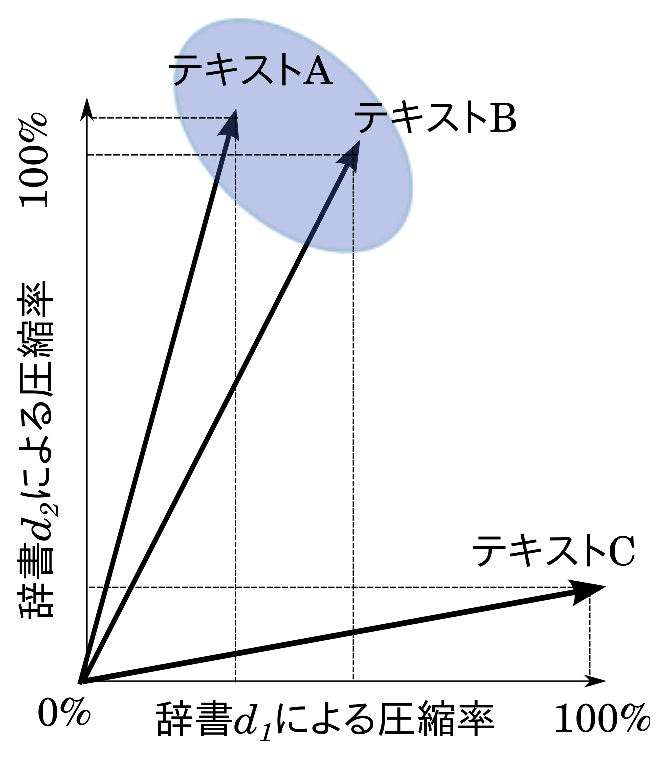
\includegraphics[width=8.5cm]{image/cv.eps}
\end{center}
\caption{圧縮率ベクトルによるテキストの特徴表現.}
\label{cv}
\end{figure}

例えば,図\ref{cv}のようにA,B,Cというオブジェクトがあった場合,2つの圧縮辞書$d_1$と$d_2$
を用いてそれらオブジェクトの特徴を2次元の圧縮率ベクトルで数値化し,
圧縮率ベクトル空間に写像する.
ここで空間上のベクトル間の距離に着目すると,AはCよりもBのほうが近い
位置にあるので,Bに対してAはCよりも似ていると言える.
PRDCではこのように,データ圧縮技術を用いて様々なファイルを特徴づける.

%つまり,$\boldsymbol{p}(D,x)$は入力テキスト$x$を基底辞書集合$D$によって圧縮して得られる
%ベクトルを表す.
%このようにPRDCでは元のオブジェクトを数値ベクトルとして表現し,

ここで,基底辞書集合$B=\{D_1,D_2,\dots,D_N\}$は,データベースから選択した$N$個のオブジェクト群
$\{T_1,T_2,\dots,T_N\}$を実際に圧縮して生成する.どのオブジェクトを利用するかはパターン
認識性能に影響を与える因子である.\cite{PRDC}では,以下のような基底辞書集合の生成方法を
提唱している.まず,$N$個のオブジェクトをランダムに選んで暫定的な圧縮特徴空間を構築する.
そして,暫定特徴空間上でデータベース内のオブジェクトをクラスタリングし,クラスタ代表となった
$N$個のオブジェクトから最終的な基底辞書集合を生成する.
この,教師なしで基底辞書を求める方法に対し,Cilibrasiら\cite{cilibrasi2007statistical}は,全てのオブジェクトクラスから均等に代表オブジェクトを選ぶ,教師ありの方法を行った.具体的には,$C$クラス分類を行うために,$N$次元の圧縮ベクトルを利用する場合には,クラスごとに$\frac{N}{C}$個のオブジェクトを選択する.
%例えば,A,Bの2つのオブジェクトがあり,Aから作られた辞書を用いて,Bを圧縮した場合,
%それが高圧縮であればAとBは似ていると考えられる.

%ここであらかじめ様々な種類のテキスト群$T=\{t_1,t_2,\dots,t_N\}$を収集しておき,
%それを圧縮することによって得られる辞書群$D=\{d_1,d_2,\dots,d_N\}$を基底辞書集合とする.
\section{辞書に基づく非類似度計算}
\ref{subsec:NCD}章で述べたNCDでは類似度を算出する際に毎回オブジェクトを圧縮するために,類似度計算の計算量が
大きい.そこで,図\ref{fig:image/Create_dictionary.eps}のように,予めオブジェクトを圧縮し,その過程で構成された圧縮辞書をオブジェクトの要約とみなし,その辞書間で距離(非類似度)を計算する手法が提案された.
辞書による非類似度として,Normalized Dictionary Distance (NDD) \cite{NDD}, Fast Compression Distance(FCD)\cite{cerra2012fast}がよく知られている.

\begin{figure}[tb]
\begin{center}
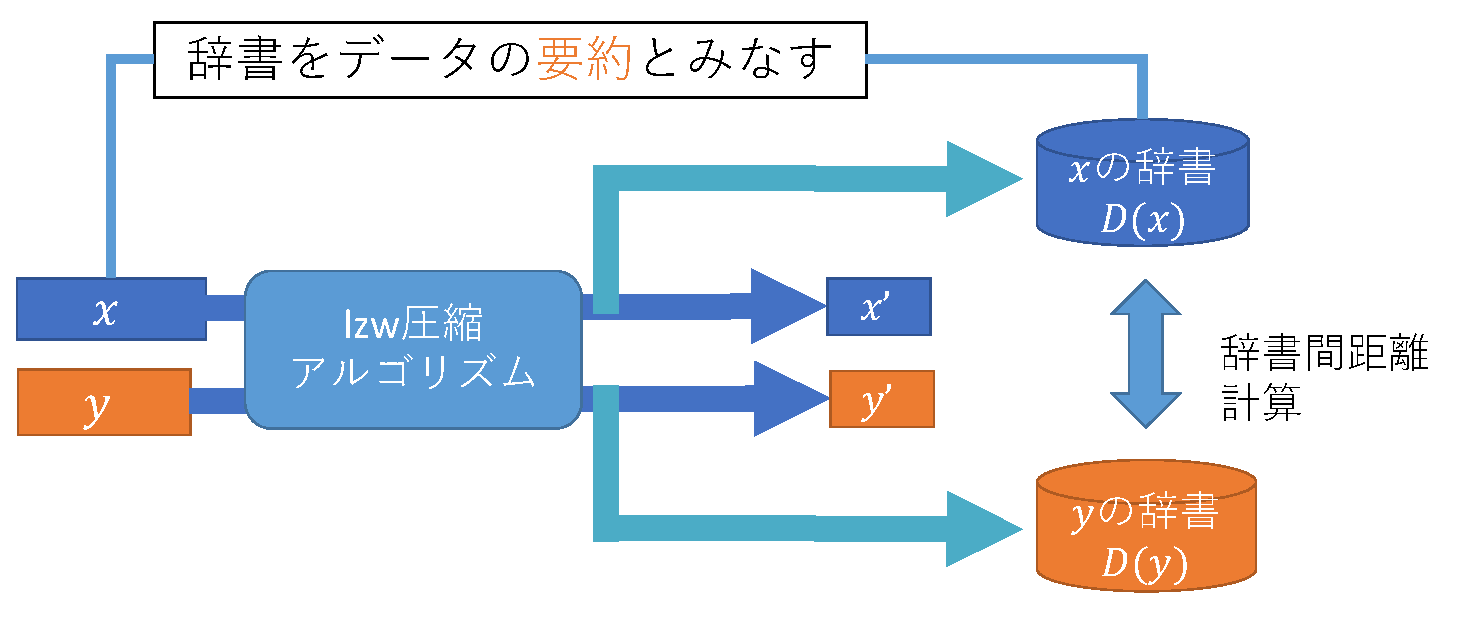
\includegraphics[clip, width=\columnwidth]{image/Create_dictionary.eps}
\caption{辞書に基づく非類似度(距離)計算}
\label{fig:image/Create_dictionary.eps}
\end{center}
\end{figure}



% LZWによる辞書構築の流れを図~\ref{fig:image/lzw.eps}に示す.
% LZWアルゴリズムによる辞書の構築は,次の手順で行う.
% 辞書には,長さ1の全ての文字が単語として登録されているものとする.
% \begin{enumerate}
% 	\item 辞書から,入力文字列に存在する最も長い単語Wを探す.
% 	\item 入力文字列中の単語WをWの符号に置き換える.
% 	\item 辞書に,入力文字列中のWとその次の1文字を結合した単語を登録する.
% 	\item 入力文字列中に符号に置き換えられていない文字が存在すれば,1に戻る.
% \end{enumerate}

%圧縮率に基づく類似度計算では,圧縮アルゴリズムにより出力される符号化文字列から特徴量を取り出し,分類を行っている.また,圧縮辞書に基づく類似度計算では,圧縮アルゴリズムにより構成される辞書から特徴量を取り出し,類似度の計算をこなっている.


%辞書に基づく非類似度(距離)計算では,オブジェクトをLZW圧縮アルゴリズムで圧縮
%した際に構成される辞書が利用される.

%辞書構築の全体的な流れは
%図\ref{fig:image/lzw.eps}のようになる.まずオブジェクトから文字列を作成する.
%オブジェクトから文字列を作成する例として,画像処理でよく用いられる方法に,水
%平スキャンがある.
%これは画像の左側から右側へ水平方向に走査し,ピクセル
%の情報を文字列に変換する方法である.

\subsection{NDD} % (fold)
\label{sub:ndd}
NDDでは,辞書を登録された単語の集合として取扱う.$D(x)$をオブジェクト$x$に対する
圧縮辞書とする.$x,y$間の距離 NDD($x,y$)は式(\ref{eq:NDD})のように定義される.
\begin{eqnarray}
\mathrm{NDD}(x,y) = \frac{ \cup(D(x),D(y)) - \min\{|D(x)|,|D(y)|\} }{ \max\{|D(x)|,|D(y)|\} }
\label{eq:NDD}
\end{eqnarray}
$|D(x)|$は$D(x)$に含まれる単語数,$\cup(D(x),D(y))$は$D(x)$と$D(y)$の和集合である.
2つの辞書が共通単語を多く含むほど$\cup(D(x),D(y))$の要素数が小さくなり,辞書間距離は小さくなる.

\subsection{NMD} % (fold)
\label{sec:nmd}
% section nmd (end)
辞書間距離の本質は,辞書を元オブジェクトの要約として用いることで計算量を削減することにある.
その一方で,辞書は元オブジェクトから情報を捨てており,この点が辞書間距離の欠点である.
そこで,Besirisらは辞書$D(x)$内の各単語が元オブジェクト$x$内に出現する回数を考慮した
辞書間距離Normalized Multiset Distance (NMD) \cite{NMD}を提案した.NMDでは,図\ref{fig:image/CalcNMD.eps}のように単語の出現回数を考慮した単語の多重集合間で距離計算をする.
ここで多重集合における単語の重複度は,出力における符号の出現回数である.(例外的に,辞書に存在するが出力には出現しない単語は,重複度1として扱う.)
\begin{figure}[tb]
\begin{center}
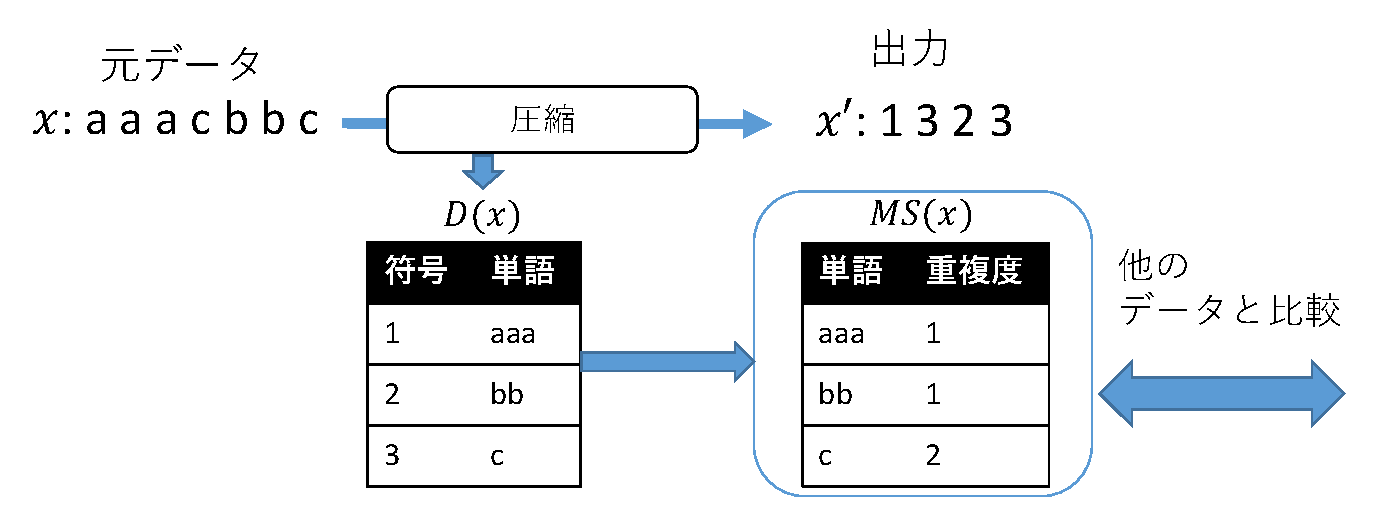
\includegraphics[clip, width=\columnwidth]{image/CalcNMD.eps}
\caption{NMD計算の流れ}
\label{fig:image/CalcNMD.eps}
\end{center}
\end{figure}

文字列$x$の辞書$D(x) = \{w_1,w_2,...,w_n\}$を順序不同の$n$個の単語の集合、$w_i$を$i$番目に抽出された単語としたとき、その多重集合$MS(x)$は次のよう
に定義される。
\begin{align}
MS(x)
&= \{D(x),m^x\} \notag \\
&= \{(w_1,m_1^x),(w_2,m_2^x),...,(w_n,m_n^x)\}
\end{align}
ここで$m_i^x$は$i$番目の単語$w_i$の出現回数であり、$m^x$は$x$中の単語出現回数を並べたリストである.$MS(x)$の要素数$|MS(x)|$は次のように定義される.
\begin{equation}
|MS(x)| = \sum_{i=1}^n m_i^x
\end{equation}

$x,y$間の距離 NMD($x,y$)は式(\ref{eq:NMD})で計算される.
\begin{equation}
\frac{|MS(x)\cup MS(y)| - \min(|MS(x)|,|MS(y)|)}{\max(|MS(x)|,|MS(y)|)}
\label{eq:NMD}
\end{equation}
式$(\ref{eq:NMD})$では,2つの多重集合$MS(x) = \{D(x),m_x\}$, $MS(y) = \{D(y),m_y\} $間で
非類似度を計算する式になっている.$MS(x)$と$MS(y)$の和集合$MS(z)= \{D(z),m_z\}=
MS(x)\cup MS(y)$は
\begin{gather}
\label{eq:x_cup_y_0}
D(z) = D(x)\cup D(y) \\\label{eq:x_cup_y_1}
m_z(w_i) = \max(m_x(w_i),m_y(w_i))
\end{gather}
として定義される。
%これらに基づき、Normalized Multiset Distance(NMD)という非類似度(距離)を以下のように定義する.


%NDDは任意のオブジェクト$x,y$から作成された辞書$D(x),D(y)$に対して次のように定義される.
%\begin{equation}
%NDD(x,y)
%\end{equation}

%\label{sub:nmd}
\cite{NMD}はNDD,FCDよりもパターン認識精度を向上させることを示した.
